\subsection{Q10.14 data 10312021 11092021 grouped by scenario \& Ethnicity}

\begin{comment}
                   EFPR        EO      EFNR     n    pvalue
(frauth, Maj)  0.361111  0.638889  0.500000  18.0  0.212946
(frauth, Min)  0.395833  0.604167  0.437500  24.0  0.246426
(icu, Maj)     0.617647  0.382353  0.676471  17.0  0.081792
(icu, Min)     0.368421  0.631579  0.473684  19.0  0.345765
(rent, Maj)    0.305556  0.694444  0.333333  18.0  0.051938
(rent, Min)    0.476190  0.523810  0.500000  21.0  0.871719
\end{comment}

\begin{table}[h]
    \centering
    \begin{tabular}{|c|c|c|c|c|c|c|}
        \hline
        scenario & Ethnicity & EFPR & EO & EFNR & n & p-value\\
        \hline
        frauth & Maj & 0.361 & \textbf{0.639} & 0.500 & 18.0 & 0.213\\
		frauth & Min & 0.396 & \textbf{0.604} & 0.438 & 24.0 & 0.246\\
		icu & Maj & \textbf{0.618} & 0.382 & \textbf{0.676} & 17.0 & 0.082\\
		icu & Min & 0.368 & \textbf{0.632} & 0.474 & 19.0 & 0.346\\
		rent & Maj & 0.306 & \textbf{0.694} & 0.333 & 18.0 & 0.052\\
		rent & Min & 0.476 & \textbf{0.524} & 0.500 & 21.0 & 0.872\\
		
        \hline
    \end{tabular}
    \caption{Grouped by scenario Ethnicity}
    \label{tab:my_label}
\end{table}
\begin{figure}[h]
    \centering
    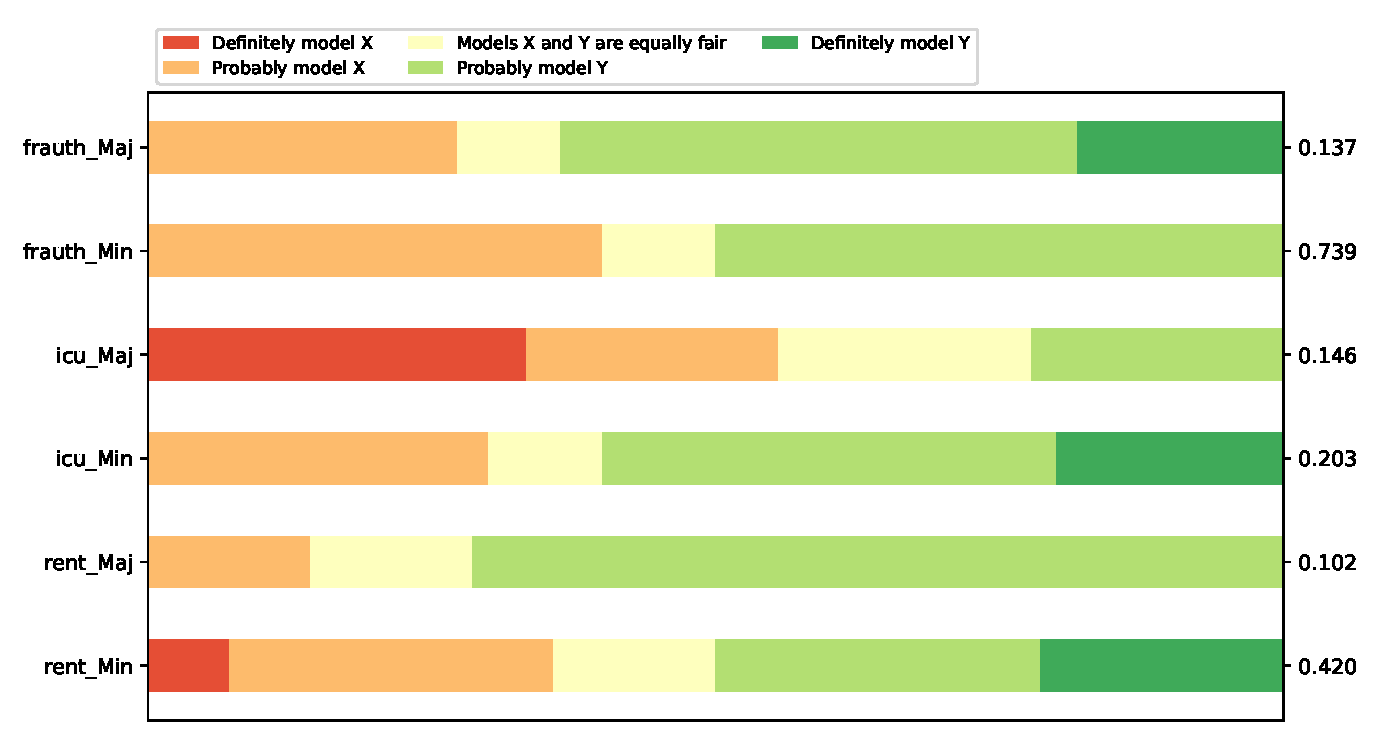
\includegraphics[width=0.8\textwidth]{figures/Q10.14/10312021_11092021/Q10.14_scenario_Ethnicity.pdf}
    \caption{Grouped by scenario \& Ethnicity}
    \label{fig:my_label}
\end{figure}
